\documentclass[11pt,letterpaper]{article}

\usepackage[T1]{fontenc}
\usepackage[utf8]{inputenc}
\usepackage{lmodern}
\usepackage{textcomp}
\usepackage{amsmath}
\usepackage{amsfonts}
\usepackage{amssymb}
%\usepackage{comment}
\usepackage{color}
\usepackage{xcolor,graphicx}
\usepackage[left=1.00in, right=1.00in, top=1.00in, bottom=1.00in]{geometry}

\usepackage[square,numbers,compress]{natbib}
\usepackage[pdftex,
pdfauthor={John J. Hopfield},
pdftitle={Unlearning has a stabilizing effect in collective memories},
pdfsubject={neuroscience},
pdfkeywords={associative memory, content-addressable memory},
pdfproducer={LaTeX},
pdfcreator={pdfTeX},
colorlinks=true,
linkcolor={red},
citecolor={green}]{hyperref} % this one has to be last

\title{`Unlearning' has a stabilizing effect in collective memories\footnote{Originally published in Nature Vol. 304, July 14, 1983}}
%\author{J.~J.~Hopfield\textsuperscript{*,\ddag}, D.~I.~Feinstein\textsuperscript{*}, and R.~G.~Palmer\textsuperscript{\dag} \\
%\textsuperscript{*}California Institute of Technology, Pasadena, California 91125, USA \\
%\textsuperscript{\dag}Duke University, Durham, North Carolina 27706, USA \\
%\textsuperscript{\ddag}Bell Laboratories, Murray Hill, New Jersey 07974, USA}
\author{J.~J.~Hopfield\footnote{California Institute of Technology, Pasadena, California 91125, USA}, D.~I.~Feinstein\footnote{Duke University, Durham, North Carolina 27706, USA}, and R.~G.~Palmer\footnote{Bell Laboratories, Murray Hill, New Jersey 07974, USA}}
\date{July 14, 1983}

\begin{document}
	\maketitle
	
	\begin{abstract}
		Crick and Mitchison\textsuperscript{\ref{ref-1}} have presented a hypothesis for the functional role of dream sleep involving an `unlearning' process. We have independently carried out mathematical and computer modelling of learning and `unlearning' in a collective neural network of $30-1,000$ neurones. The model network has a content-addressable memory or `associative memory' which allows it to learn and store many memories. A particular memory can be evoked in its entirety when the network is stimulated by any adequate-sized subpart of the information of that memory\textsuperscript{\ref{ref-2}}. But different memories of the same size are not equally easy to recall. Also, when memories are learned, spurious memories are also created and can also be evoked. Applying an `unlearning' process, similar to the learning processes but with a reversed sign and starting from a noise input, enhances the performance of the network in accessing real memories and in minimizing spurious ones. Although our model was not motivated by higher nervous function, our system displays behaviours which are strikingly parallel to those those needed fro the hypothesized role of `unlearning' in rapid eye movement (REM) sleep. \\
	\end{abstract}

	In the most symmetric form of collective memory in our dynamic neural network\textsuperscript{\ref{ref-2}}, each neurone, $j$, has two states, and is described by a variable $\mu_j = \pm1$. The instantaneous state of the system of $N$ neurones can be thought of as an $N$-dimensional vector have components $\mu_i$ of size 1. The neurones are interconnected by a network of synapses, with a synaptic strength $T_{ij}$ from neurone $j$ to neurone $i$. The instantaneous input to neurone $i$ is
	\begin{equation}
		\text{input to } i=\sum_{i\ne1} T_{ij} \mu_j
	\end{equation}
	where $\mu_j$ is the present state ($\pm1$) of neurone $j$. The neural state of the system changes in time under the following algorithm. Each neurone $i$ interrogates itself at random in time, but at a mean rate $W$, and readjusts its state, setting $\mu_i=\pm1$ according to whether the input to $i$ at the moment is greater or less than zero. The neurones act asynchronously.
	
	This algorithm defines the time evolution of the state of the system. For any symmetric connection matrix, there are stable states of the network of neurones, in which each neurone is either `on' and has an input $\geq0$ or `off' and has an input $<0$. These stable states will not change in time. Starting from any arbitrary initial state, the system reaches a stable state and ceases to evolve in a time of $\sim3/W$.
	
	The stable states of the system can be arbitrarily assigned by an appropriate choice of $T_{ij}$. Suppose $n$ different $N$-dimensional state vectors
	\begin{equation}
		\mu_{i}^{s}\}_{i=1}^{N} s=1 \text{ to } n\leq0.25N
	\end{equation}
	are able to be stable states of the system. If these state vectors are sufficiently different, and if the synaptic connection matrix $T_{ij}$ is given by
	\begin{equation}
		T_{ij}=\sum_{s} \mu_{i}^{s} \mu_{j}^{s};T_{ii}=0; i\neq j
	\end{equation}
	then the states $\mu^{s}$ will be stable states of the system.
	
	This network now functions as an associative memory. If started from an initial state which resembles somewhat state $\mu^{t}$ and which resembles other $\mu^{s}(s\neq t)$ very little, the state will evolve to the state $\mu^{t}$. The state $\mu^{s}$ are evokable memories, and the system correctly reconstructs an entire memory any initial partial information, as long as the partial information was sufficient to identify a single memory. Detailed properties of the collective operation of this network have been described previously\textsuperscript{\ref{ref-2}}.
	
	The form of the $T_{ij}$ matrix can be described as an incremental learning rule. To learn a new memory $\mu^{\text{new}}$, increment $T_{ij}$ by
	\begin{equation}
		\text{learn } \mu^{\text{new}} \Delta T_{ij}= \mu_{i}^{\text{new}} \mu_{j}^{\text{new}}
	\end{equation}
	In biology or circuits, this would be done by placing the system in state $\mu^{\text{new}}$---for example, driven by external inputs---and enabling a learning process that allows all $T_{ij}$ to increment. The information needed by each synapse is local---the increment for synapse $ij$ does not depend on the global structure of the new state or past memories, but only on $\mu_{i}^{\text{new}}$ and $\mu_{j}^{\text{new}}$.
		
	Under this algorithm, when random starting stares are chosen, some stored memories are much more accessible than others, that is, considerably larger numbers of randomly chosen initial states lead to some memories than to others. This is a vagary of the particular set of memories which have been learned. It occurred to us that it would be possible to reduce this unevenness of access (which can be intuitively described as the ``50\% of all stimuli remind me of sex'' problem) by `unlearning'.
	
	Specific unlearning was implemented by choosing starting states at random; when a final equilibrium state $\mu^{f}$ was reached it was weakly unlearned by the incremental change
	\begin{equation}
		\text{unlearn } \mu^{f} \Delta T_{ij} = - \epsilon \mu_{i}^{f} u_{j}^{f} , 0 < \epsilon \ll 1
	\end{equation}

	Figure \ref{figure-1} illustrates the effect of unlearning on the accessibility of five stored memories in a set of $32$ neurones. Accessibility is quantitatively defined as the fraction of random initial states leading to a particular final stable state or group of states. The unevenness of the lines is due in part to statistical noise in the simulation. The accessibility of the nominal assigned memories initially ranges over a factor of $3$, but converges with unlearning to a spread of only a factor of $1.4$. Thus the accessibility is much more uniform (or in Crick-Mitchison terms, the relative stability of the modes made more uniform) after specific unlearning, and the system will have functionally improved recall.
	
	\begin{figure}[h]
		\begin{center}
			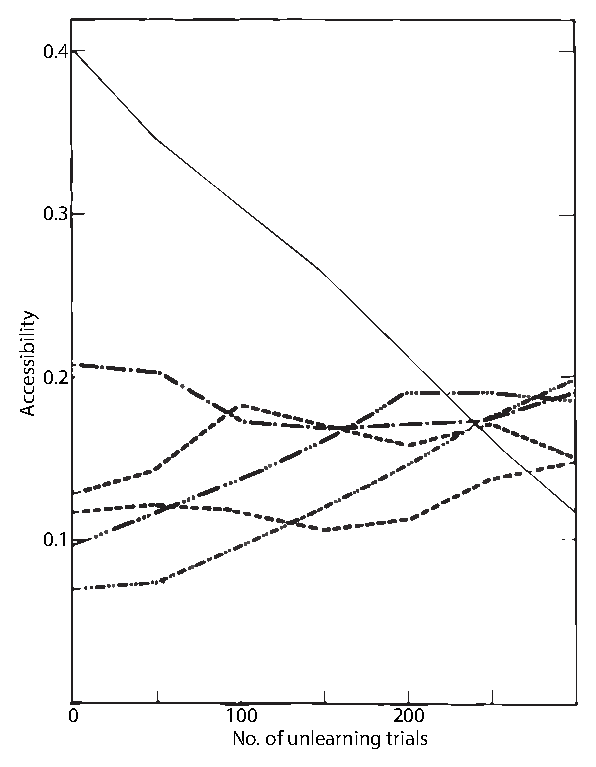
\includegraphics[width=0.5\linewidth]{Hopfield-1983-Figure-1.eps}
		\end{center}
		\caption{The fraction of random starting states which leads to particle memories (accessibility). The five dashed lines are the five nominal memories. The solid line is the total accessibility of all spurious memories. In these trials $\epsilon$ was set at $0.01$.} \label{figure-1}
	\end{figure}

	In our model the storage of a set of assigned memories in $T_{ij}$ also produces a set of spurious stable states which were not inserted as memory states. One of the strong effects of unremembering is to reduce the total accessibility of spurious states, as shown by the solid line in Fig.~\ref{figure-1}.
	
	The qualitative reason for the success of unlearning comes from the behaviour of the `energy' $E$, defined for any state $\mu$ as
	\begin{equation}
		E=- \sum_{i \ne j} \sum_{j} T_{ij} \mu_{i} \mu_{j}
	\end{equation}
	The change of neural state with time according to the asynchronous algorithm monotonically decreases $E$ until a final stable state is reached---either a stored memory or a spurious memory. Any stable state $\mu^{m}$ has, for a given $T_{ij}$, an energy $E^{m}$. There is a strong tendency for the states having the deepest energy valleys to collect from the largest number of random starting states, that is, deep valleys are also broad. When a final state $\mu^{f}$ is unlearned, its energy $E^{f}$ is specifically raised and its valley of collection diminished relative to other states. While this argument indicates why accessibility of stored memories should be made more nearly even by unlearning, only a detailed analysis shows why the spurious states should be so sensitive to it. Too much unlearning will ultimately destroy the stored memories.
	
	We have identified a class of spurious states, which in their most elementary form have their origin in triples. As an example on $16$ neurones
	\\
	\\
	\begin{tabular}{cc}
		Memory 1 & $++++----|++-+-+--$ \\ 
		Memory 2 & $++++----|--+-+-++$ \\ 
		Memory 3 & $++--++--|+--++--+$ \\ 
		Spurious memory & $++++----|+--++--+$ \\ 
	\end{tabular}
	\\
	\\
	The stability of the spurious memory is enhanced if the first half of memory $3$ is weakly correlated with memories $1$ and $2$. Mathematical analysis of the statistical stability of such spurious states shows that they are typically less stable than the assigned memories, and that the stability will also depend on correlations with other memories. The nature of these spurious states can be described by analogy in terms of higher level function by the example
	\\
	\\
	\begin{tabular}{cc}
		Memory 1 & Walter, white \\ 
		Memory 2 & Walter, black \\ 
		Memory 3 & Harold, grey \\ 
		Spurious memory & Walter, grey \\ 
	\end{tabular}
	\\
	\\
	where grey is taken as a category equally resembling black and white. This spurious state is more stable when `Harold' and `Walter' have a significant correlation---perhaps `Harold' and `Harry'. These particular spurious states are not simply transitive logical associations of the form $A\leftrightarrow B$, $B\leftrightarrow C$; $\rightarrow A\leftrightarrow C$. They are truly spurious `illogical' associations, but perhaps `plausible' as they come from correlations in the structure of memories.
	
	In our simple system, unlearning improves memory function by the equalization of accessibility and the suppression of spurious memories. We asked whether other simple algorithmic changes such as clipping the $T_{ij}$ matrix or a threshold effect produce an equivalent improvement in memory performance. These two do not, presumably because they lack the essential element of the present scheme, that is, the feedback via the algorithm of information about the accessibility of particular states. We believe the results found will be insensitive to whether the state component values are taken as $0$ or $1$ or $\pm 1$.
	
	The REM sleep hypothesis of Crick and Mitchison\textsuperscript{\ref{ref-1}} refers to higher level processing. Our example illustrates that from a mathematical viewpoint the general idea could work as they described. If the Crick-Mitchison hypothesis is correct, one might ask about correlations between the structure of the spurious linkages in modelling and the strange associations present in dreams.
	
	We thank F.~Crick and D.~Willshaw for discussions. This work was supported in part by NSF grant DMR-8107494 and by the System Development Foundation.
	\\
	\\
	Received 31 December 1982; accepted 15 May 1983.
	
	\subsubsection*{References}
	\begin{enumerate}
		\item Crick, F.~C.~\& Mitchison, G.~\textit{Nature} \textbf{304}, 111--114 (1983). \label{ref-1}
		\item Hopfield, J.~J.~\textit{Proc.~natn.~Acad.~Sci.~U.S.A.}~\textbf{79}, 2554--2558 (1982). \label{ref-2}
	\end{enumerate}
\end{document}